\section{BCOoL Framework}
\label{section:bcoollengbench}
In this section, we present the \bcool framework that is the integration of \bcool into the GEMOC studio~\footnote{http://www.gemoc.org}. The GEMOC Studio integrates technologies based on Eclipse Modeling Framework (EMF)~\footnote{http://eclipse.org/modeling/emf/} adequate for the specification of executable domain specific modeling languages. It includes a \emph{language workbench} to design and implement tool-supported xDSMLs and a \emph{modeling workbench} where the xDSMLs are automatically deployed to allow system designers to edit, execute, simulate, and animate their models~\cite{ttc15bib}. \bcool takes advantages of this collaborative environment by adding coordination facilities. In this section, we elaborate on the workflow presented in Figure~\ref{fig:proposedworkflow}. An integrator uses the language workbench to develop \bcool operators to specify coordination patterns between languages. Then, a system designer can use these operators in the modeling workbench to execute and verify coordinated models. We begin this section by showing how the language workbench is used to develop \bcool operators. In particular, we develop the operator for the running example (see Listing~\ref{lst:bcoolrunningexample}). Then, in the modeling workbench, we use this operator to execute and verify the models of the coffee machine. 
\begin{figure}[h]
	\begin{center}
		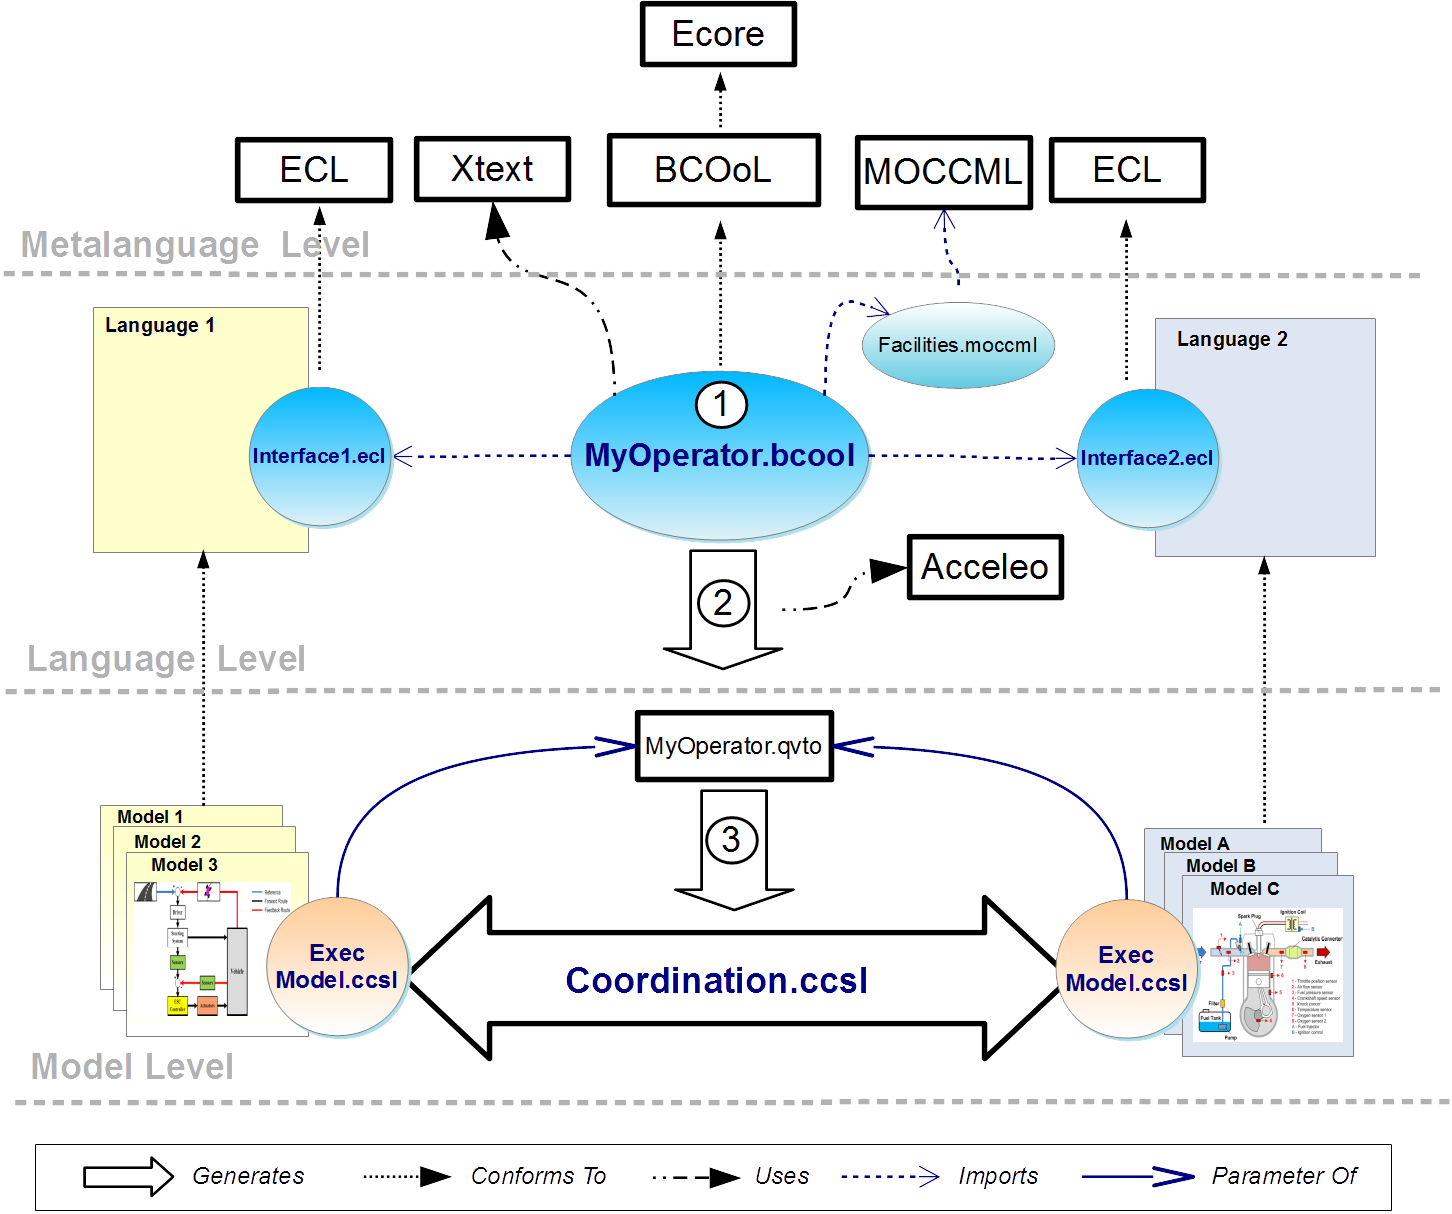
\includegraphics[width=1\textwidth]{bcool/figs/bcooltechnos}
		\caption{Overview of the \bcool framework}
		\label{fig:bcooltechnos}
	\end{center}
\end{figure}

\bcool is developed as a set of plugins based on the EMF. The top of Figure~\ref{fig:bcooltechnos} illustrates the technologies used to implement \bcool into the language workbench. For example, the \bcool abstract syntax has been developed using Ecore (\ie the meta-language associated with EMF) and the textual concrete syntax has been developed in Xtext~\footnote{http://eclipse.org/Xtext/} thus providing advanced editing facilities. When languages are deployed into the language workbench, an integrator can define a new \bcool specification and then import the language behavioral interfaces that are automatically deployed (Figure~\ref{fig:bcooltechnos}: step 1). Also, the language workbench provides \moccml thus helping the integrator to specify relations and expression. For the running example, we use the TFSM and Activity languages that are integrated into the studio. Then, we use \bcool to specify the Listing~\ref{lst:bcoolrunningexample}.   
	\begin{lstlisting}[language=bflow,
	caption={\bflow specification for the models of the coffee machine},
	label={lst:bflowcoffeemachine}, 
	basicstyle=\scriptsize\ttfamily, backgroundcolor=\color{LGrey}, numbers=left, xleftmargin=2pt]
	BCOoLFlow CoffeeMachine
	ImportBCOoL  "TFSMAndActivity.bcool" ;
	Model CoffeCoin "coffeecoin.tfsm"
	Model CoffeeAlgorithm "coffeeAlgorithm.ad"
	Flow 
	applies SyncFSMEventsAndActions between (CoffeeAlgorithm, CoffeCoin);
	end Flow;
	\end{lstlisting}


In the modeling workbench, a system designer can use \bcool operators to automate the generation of a coordination model. Also, such a model of coordination can be executed and verified. To ease the task of a system designer, we provide a simple language named \bflow. With \bflow, a system designer specifies what operators are applied on which models (Figure~\ref{fig:bcooltechnos}: step 2). For example, Listing~\ref{lst:bflowcoffeemachine} shows the simple \bflow specification for the models of the coffee machine. The \bflow specification begins by importing the \bcool specification that will be used. Then, it specifies the models that will be coordinated. For the running example, this corresponds with the TFSM named \emph{CoffeeCoin} and the Activity named \emph{CoffeAlgorithm}. Afterwards, the specification contains \emph{Flows} that defines what operator is used and on which models. For instance, in Listing~\ref{lst:bflowcoffeemachine}, line 6 specifies that the operator named SyncFMEventsAndActions will be applied between the models CoffeeCoin and CoffeeAlgorithm. The specification, however, can contain several flows. We discuss this in the next chapter.   

In the modeling workbench, the \bflow specification is used by the \emph{Gemoc Coordinated Execution Engine} to generate a model of coordination in \ccsl and then execute the coordinated system (see Figure~\ref{fig:bcooltechnos}). We automate the generation of the coordination by relying on Acceleo\footnote{http://www.eclipse.org/acceleo/} and QVTo\footnote{https://projects.eclipse.org/projects/modeling.mmt.qvt-oml}. An acceleo transformation is used to translate the \bcool specification into a QVTo transformation. Then, the QVTo transformation can be applied between models to generate the coordination specification in \ccsl. These steps have been automated by relying on a set of plugins that are integrated into the modeling workbench. We illustrate the use of the Coordinated Execution Engine by executing the models of the coffee machine. First, we configure the launcher that contains information about the \bcool specification, the \bflow specification and the configuration launcher for each model (see Figure~\ref{fig:execenginemenu}). Once launched, the engine provides several options to drive the execution of the models. For instance, it enables a system designer to select the next valid execution step (Figure~\ref{fig:runningworkbench}: point 3). Also, the workbench provides the animation of models (Figure~\ref{fig:runningworkbench}: point 4). 

In addition, the generated \ccsl specification (Figure~\ref{fig:runningworkbench}: point 1) can be analyzed by using \ccsl tools. For example, the modeling workbench offers the possibility to obtain by exploration quantitative results on the scheduling state-space of the coordinated system. The exploration of all schedules can be captured explicitly in a state space graph as presented~\ref{?}. Any cyclic path in this graph (starting from the initial configuration) represents a valid schedule of the model. The state space is always computable if the behavior of models are finite.

\begin{figure}[h]
	\centering
	\subfigure[Gemoc Coordinated Execution Engine launcher]{
		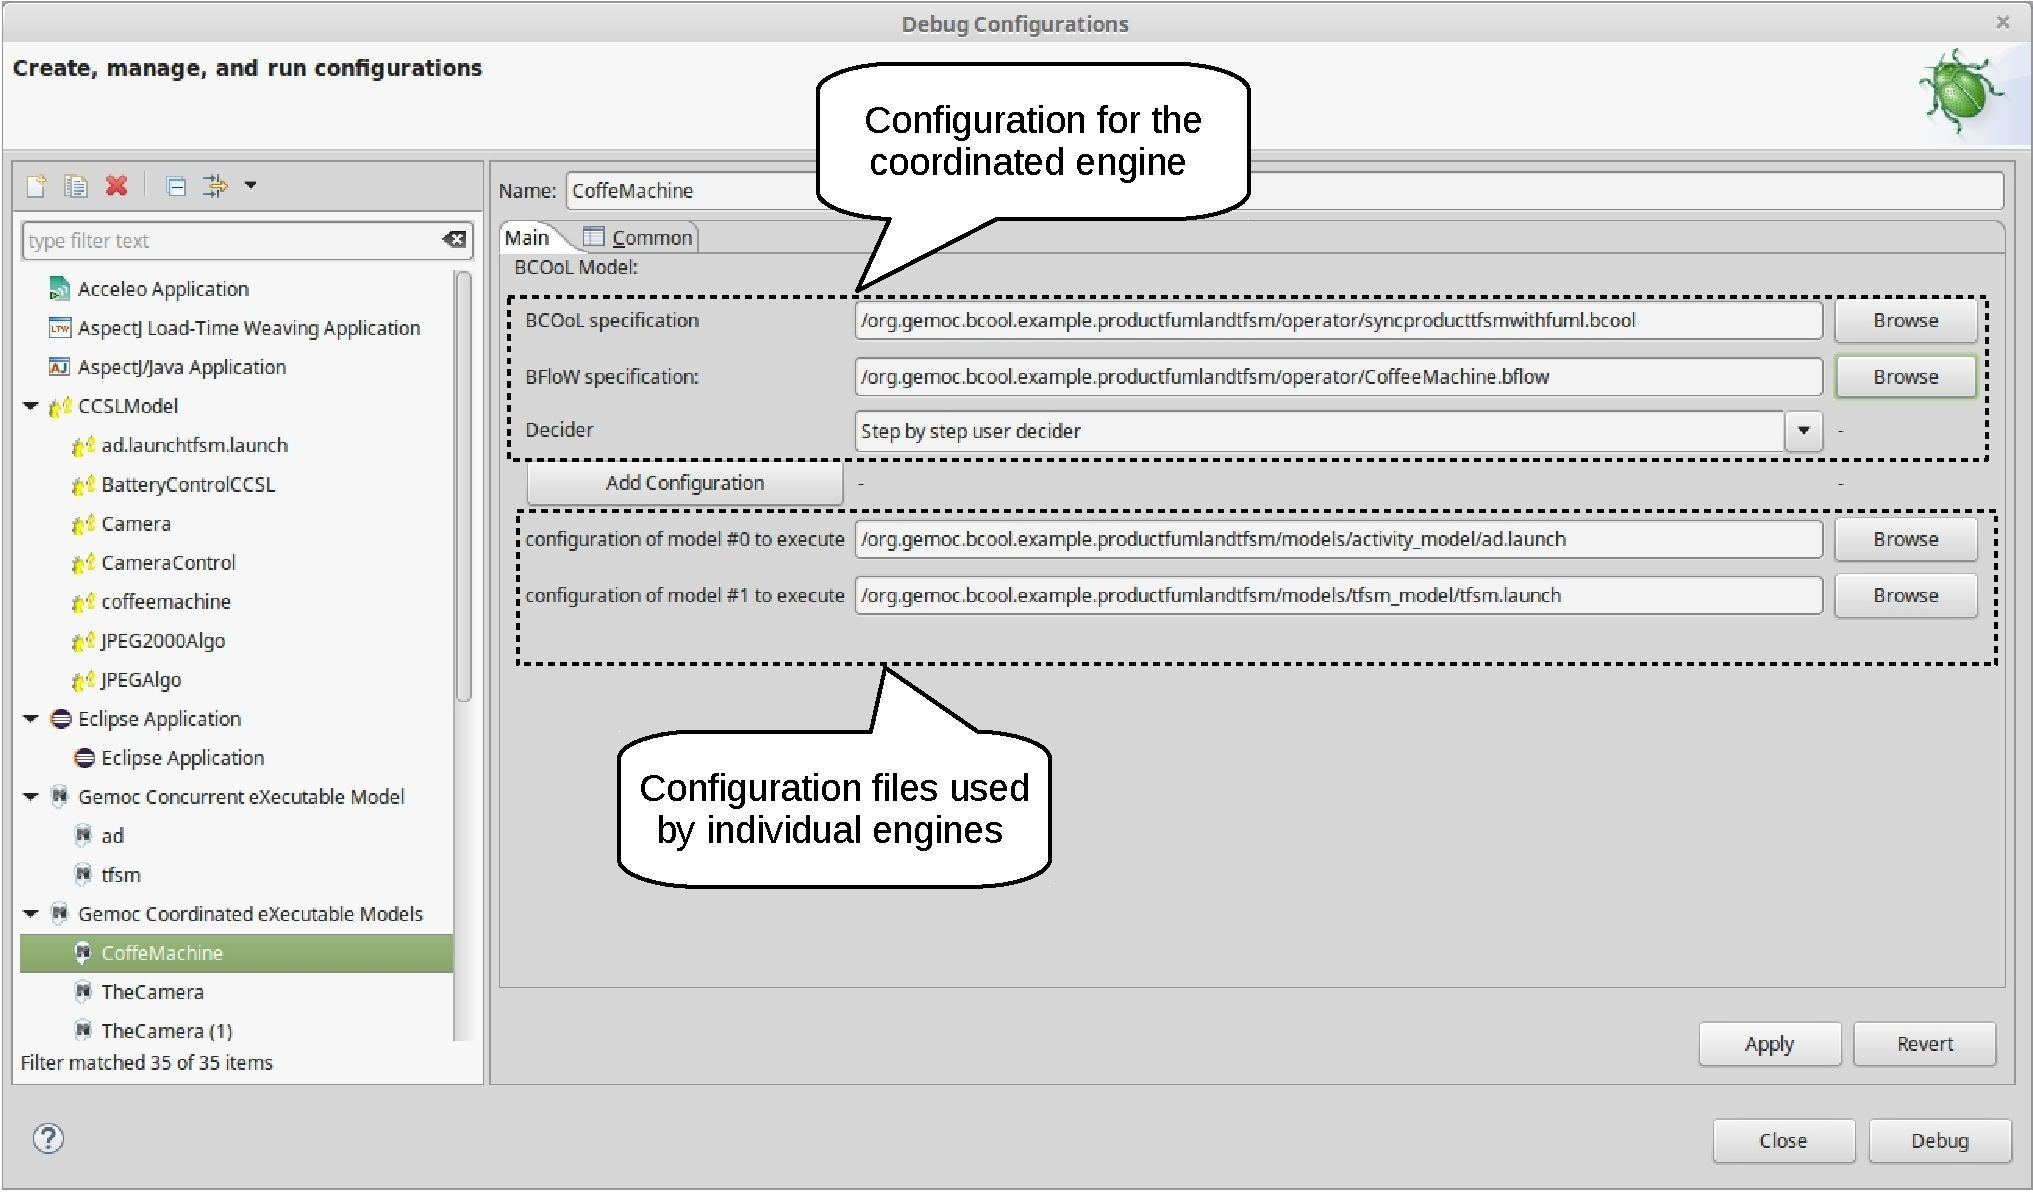
\includegraphics[width=.5\textwidth]{bcool/figs/execenginemenu}
		\label{fig:execenginemenu}
	}
	\subfigure[Coordinated Execution of the models of the Coffee Machine]{
		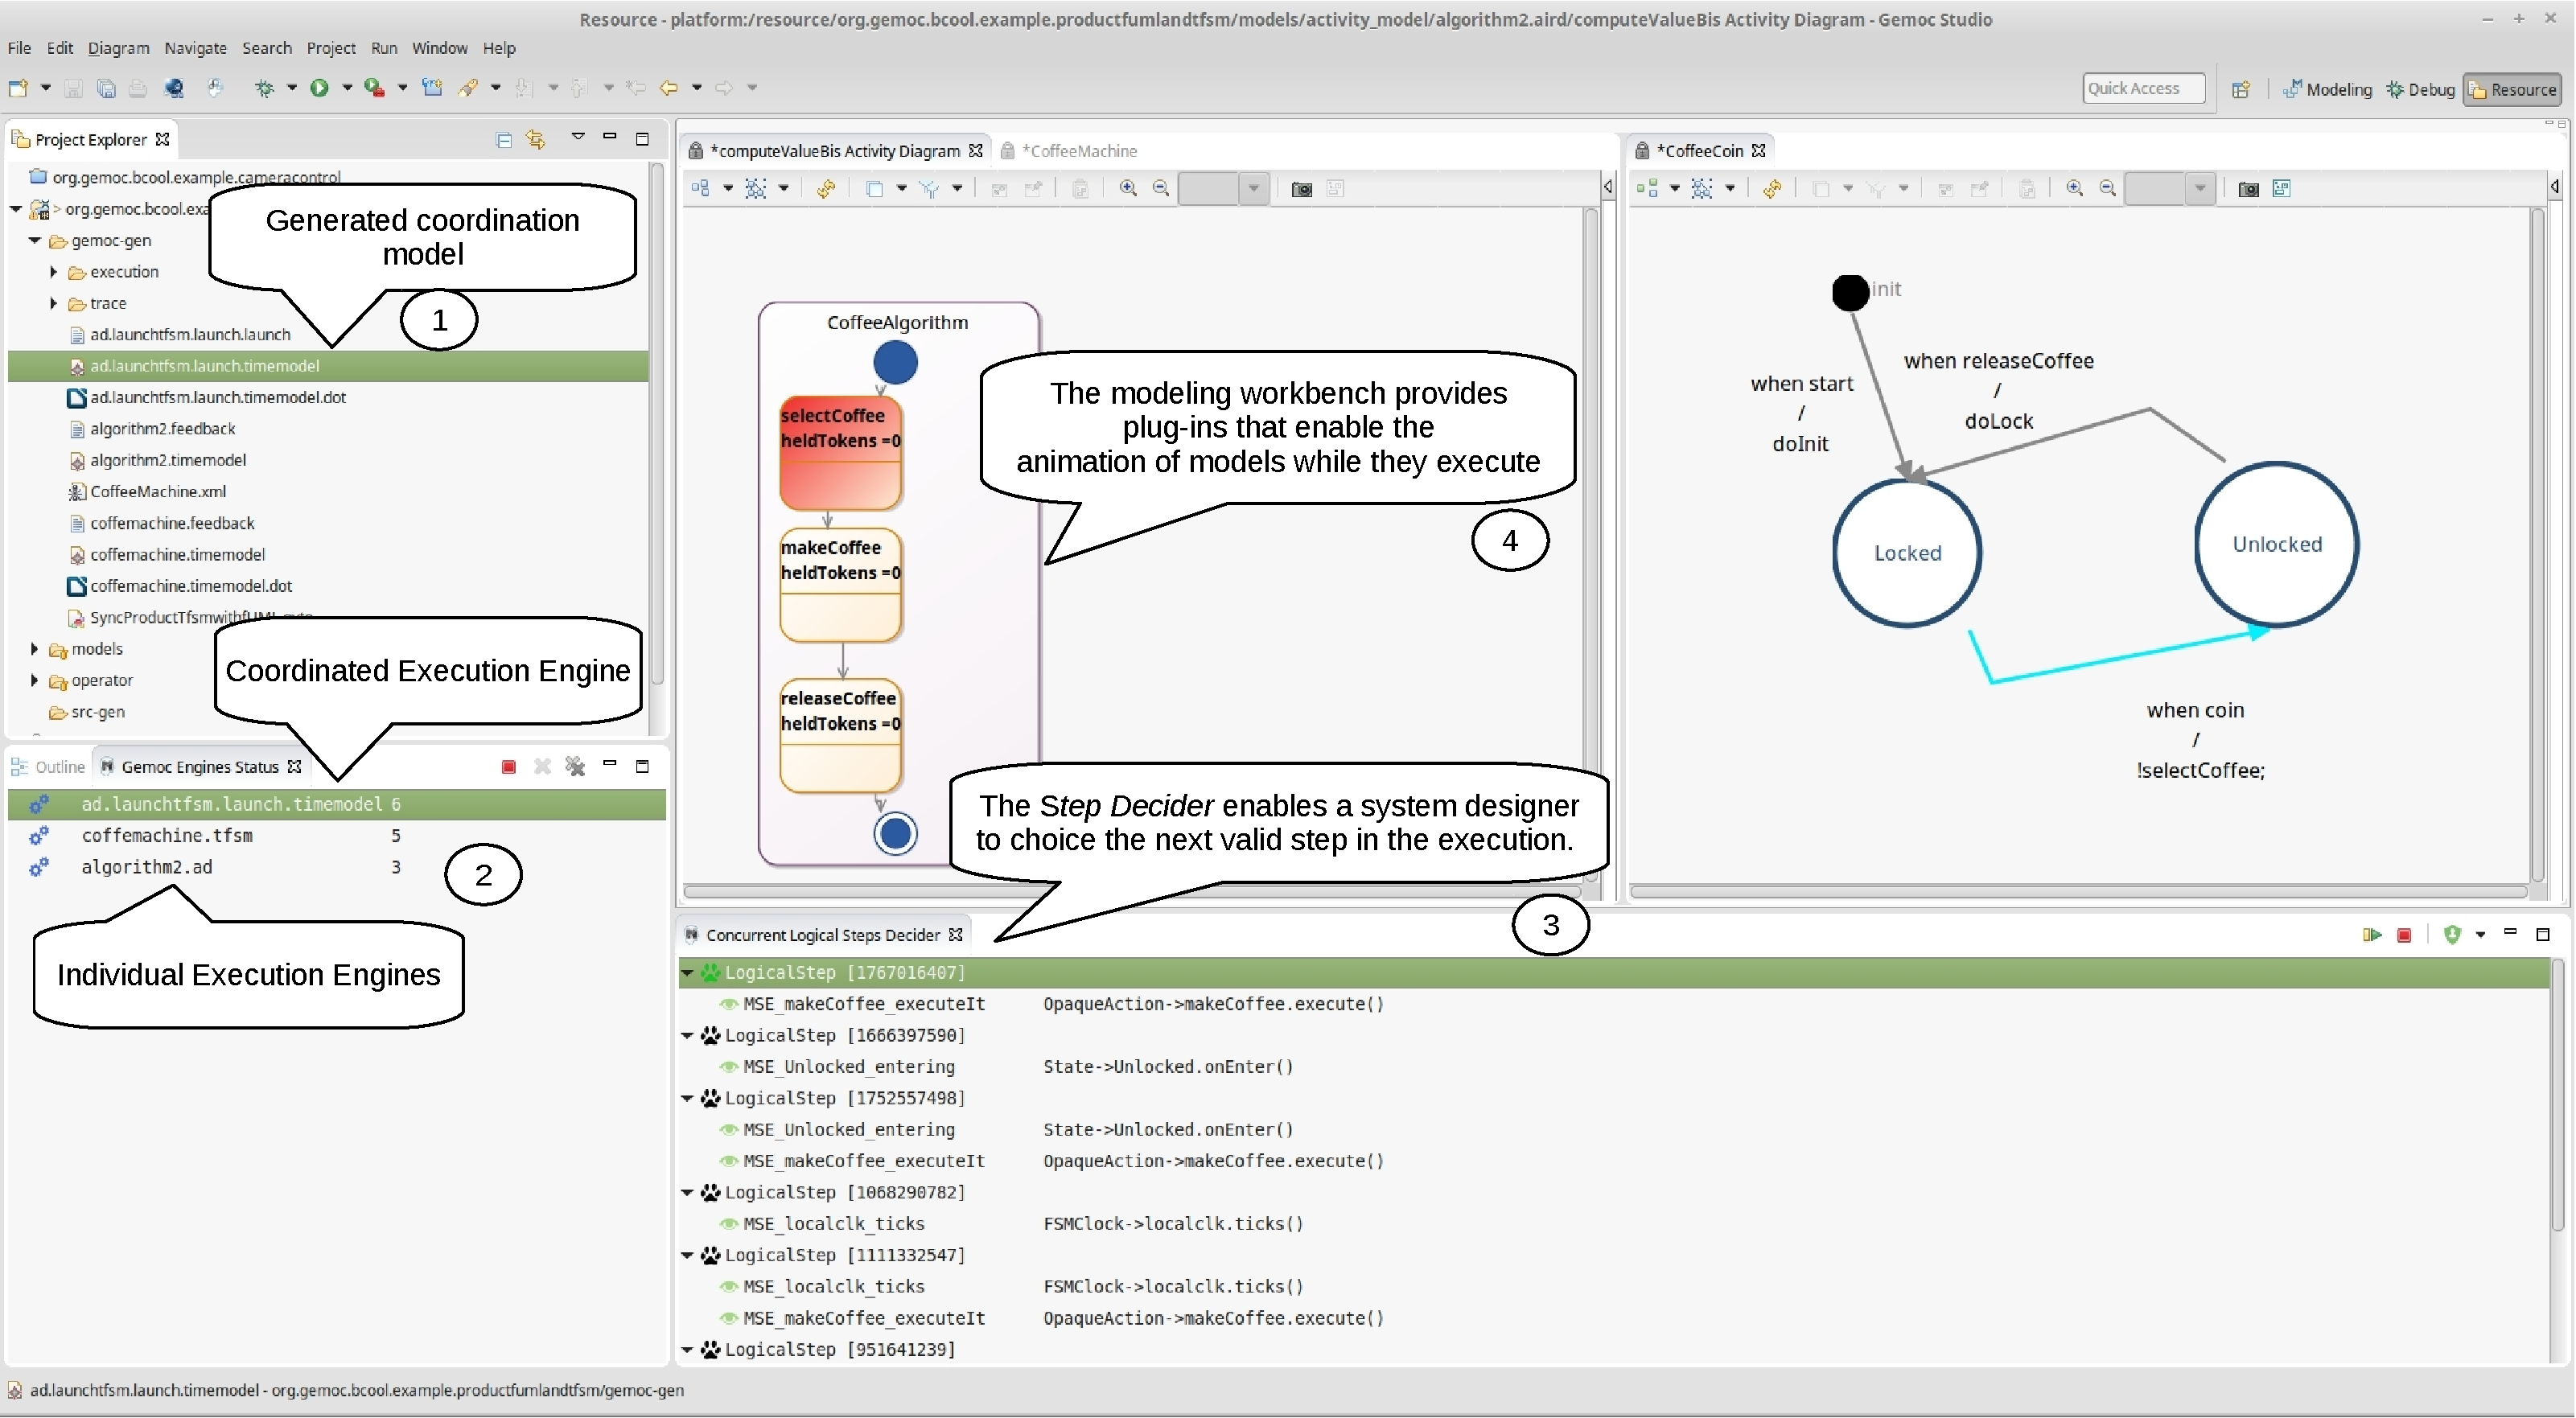
\includegraphics[width=.7\textwidth]{bcool/figs/runningworkbench}
		\label{fig:runningworkbench}
	}
	\caption[]{Coordinated Execution of models in the Modeling Workbench}
	\label{fig:subfigureExample1}
\end{figure}

\bcool is hosted on Github~\footnote{http://github.com} as part of the GEMOC project~\footnote{http://github.com/gemoc/coordination}. In addition, we built a website that contains more examples with full descriptions~\footnote{http://timesquare.inria.fr/BCOoL}. For example, it contains a video that presents the whole flow of the coffee machine example. Furthermore, the project is included into the GEMOC studio as a deployable example. To try it, it is only necessary to download the studio, and then to create a new example project. 

In this section, we have presented that current integration of \bcool into the GEMOC studio that we named the \bcool framework. The framework eases the task of integration by allowing integrators to develop operators between languages. Then, a system designer can use these operators to coordinate and execute their models. In the next section, we compare our approach with coordination languages and coordination frameworks.  

%\bcool is developed as set of plugins for Eclipse Modeling Framework (EMF)\footnote{http://www.eclipse.org}. Its abstract syntax has been developed using Ecore (\ie the meta-language associated with EMF) and the textual concrete  syntax has been developed in Xtext, thus providing advanced editing facilities (see Figure~\ref{fig:bcooltechnos}). A \bcool specification is defined between languages by relying on its language behavioral interface made of \dse. To get the \dse, the \ecl specification of each language must be imported (Figure~\ref{fig:bcooltechnos}: point 1). From a \bcool specification, the generation of the coordination between models has been automated by relying on two technologies: Acceleo\footnote{http://www.eclipse.org/acceleo/} and QVTo\footnote{https://projects.eclipse.org/projects/modeling.mmt.qvt-oml}. The acceleo transformation translates the \bcool specification into a QVTo transformation (Figure~\ref{fig:bcooltechnos}: point 2). The transformation can be applied between models to generate the coordination specification in \ccsl (Figure~\ref{fig:bcooltechnos}: point 3).    
	

	
%These technologies has been integrated into the GEMOC Studio, an Eclipse package atop EMF, which includes both a \emph{language workbench} to design and implement tool-supported xDSMLs, and a \emph{modeling workbench} where the xDSMLs are automatically deployed to allow system designers to edit, execute, simulate, and animate their models. In this context, \bcool takes advantages of this collaborative environment by adding coordination facilities. 

%\begin{figure}[h]
%	\begin{center}
%		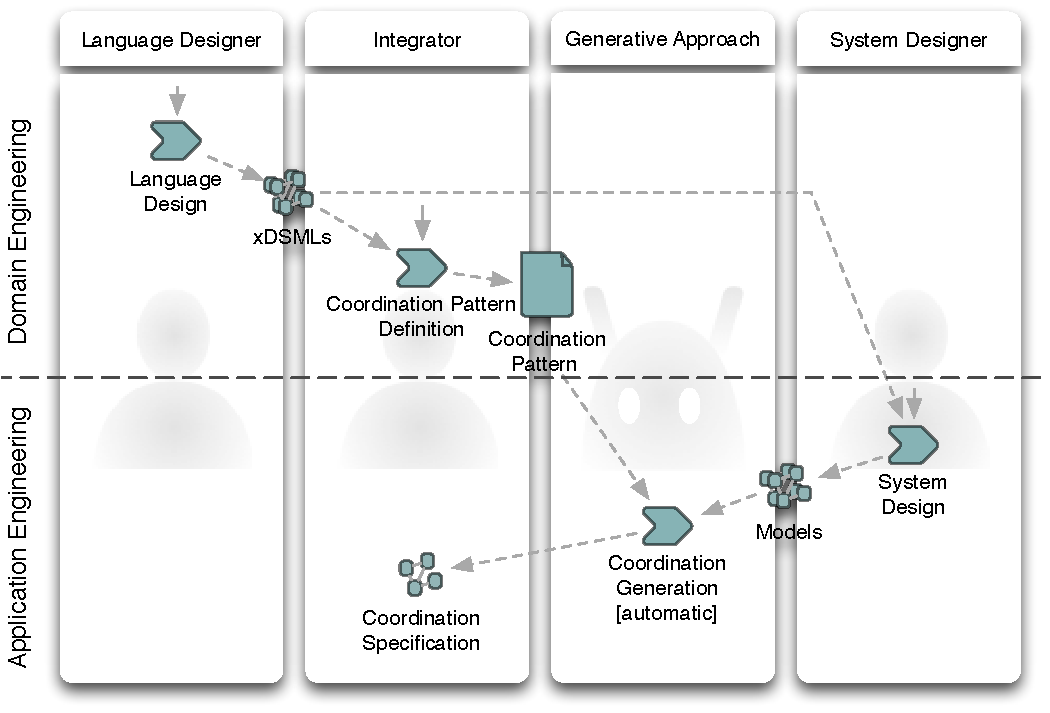
\includegraphics[width=.6\textwidth]{bcool/figs/process}
%		\caption{The Proposed Workflow}
%		\label{fig:proposedworkflow}
%	\end{center}
%\end{figure}

%Based on the GEMOC studio, Figure~\ref{fig:proposedworkflow} illustrates the proposed workflow. Such a workflow relies mainly in two stakeholders: an integrator that uses the language workbench and an system designer that uses the model workbench. 

%In the language workbench, an integrator develop operators by relying on the deployed languages. The \bcool specification can import the language behavioral interface that are automatically deployed into the workbench. To build its own libraries, the workbench provides \moccml thus helping the integrator to specify EventRelations and EventExpression. 

%Operators are automatically deployed into the modeling workbench and can be used by a system designer to generate the coordination. This task is automated by relying on a set of plugins\footnote{\todo{I have to talk about how the operators are applied by the plugin, this is not evident!}}. The workbench provides several tools to perform verification activities \eg execution and animation, space-state exploration, etc.  

%To summarize, a \bcool developer (\ie integrator) develops a set of operators by relying on the language behavioral interface (\ecl) and libraries (\moccml). Then, a \bcool user (\ie system designer) applies these operator on his models to: 
%		\begin{itemize}
%			\item Generate a coordination specification.
%			\item Perform execution and verification activities.
%		\end{itemize}

%We implement the running example in the GEMOC studio. We rely on the languages TFSM and Activity that are integrated into the study. Then, we use \bcool to specify the operator in Listing~\ref{lst:bcoolrunningexample} (Figure~\ref{fig:screenbcool}: point 1). In the model workbench, we build the models of the coffee machine: a TFSM named \emph{CoffeeCoin} and an Activity named \emph{CoffeeAlgorithm} (Figure~\ref{fig:screenbcool}: point 2). Then, we use the workbench to execute, verify and animate the coordinated models. In particular, Figure shows the animation proposed by Sirius.   

%\begin{figure}[h]
%	\begin{center}
%		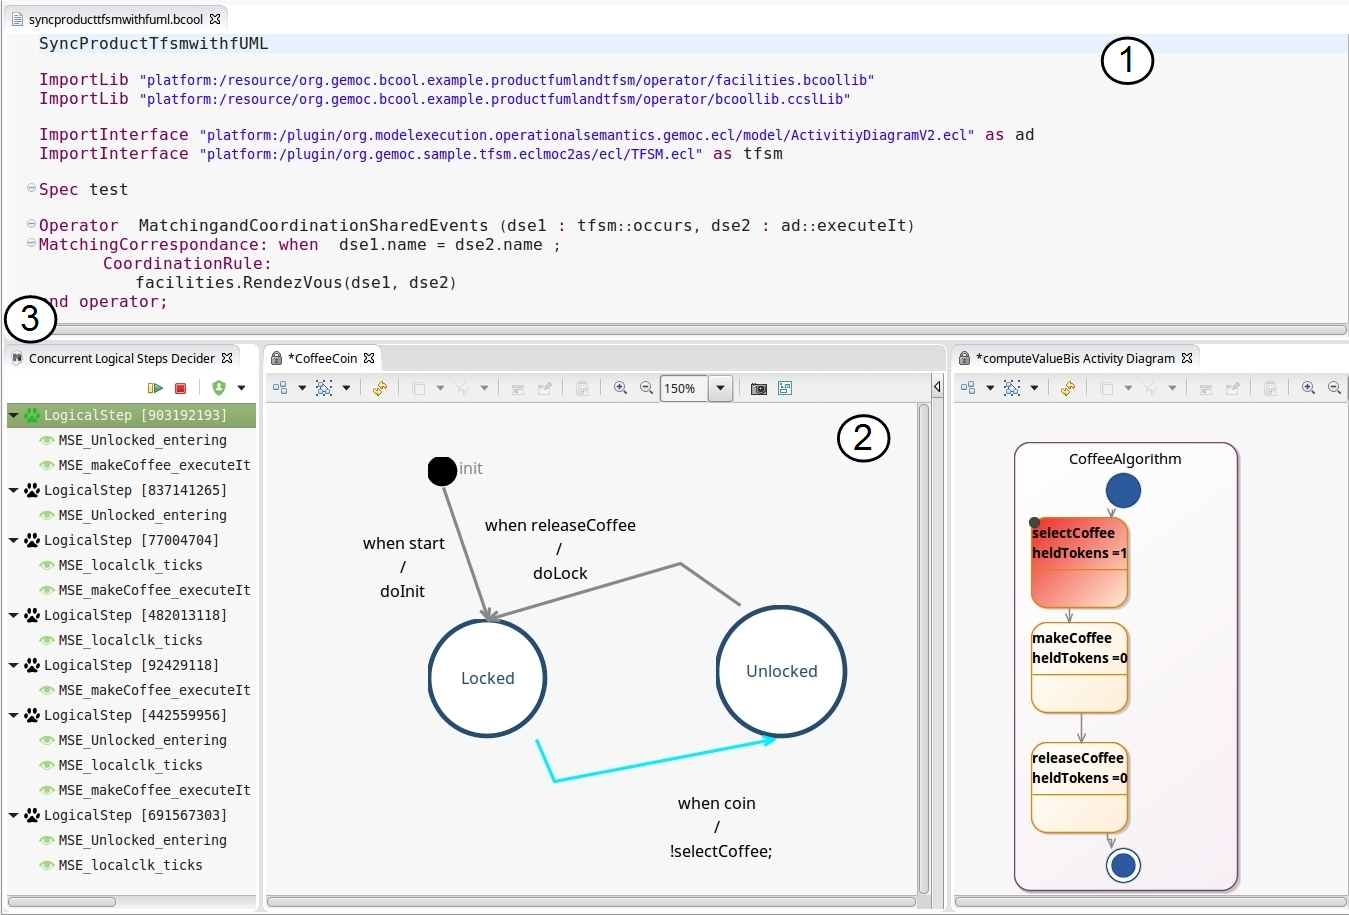
\includegraphics[width=.6\textwidth]{bcool/figs/bcoolscreen.png}
%		\caption{Screenshot}
%		\label{fig:screenbcool}
%	\end{center}
%\end{figure}

%A video presenting the whole flow can be found on the companion website~\footnote{http://timesquare.inria.fr/BCOoL}, which also contains more examples with full descriptions. These examples are hosted in Github~\footnote{http://github.com} at BCOoLExamples~\footnote{http://matiasvara.github.io/BCOoLExamples/}. The \bcool code is hosted in the open source project Gemoc~\footnote{http://github.com/gemoc/} thus making the project fully available.

%\subsection{Flow by using the plugins}
%\subsection{Flow by using ANT}
%	\begin{itemize}
%		\item Ant\footnote{http://www.eclipse.org/eclipse/ant/}
%		\item Operational QVT Ant tasks let you launch QVTO transformations from the Ant script.
%		\item The flow can be implemented by using Ant.
%		\item This enables to define explicitly how a \bcool specification is invoked. 
%		\item However, the specification of a ANT script must be partially defined by the user. For instances, several parameters must be defined by the user, \eg model paths, generated timemodel. 
		  
%	\end{itemize}


 % \begin{figure}[h]
  %	\begin{center}
  %		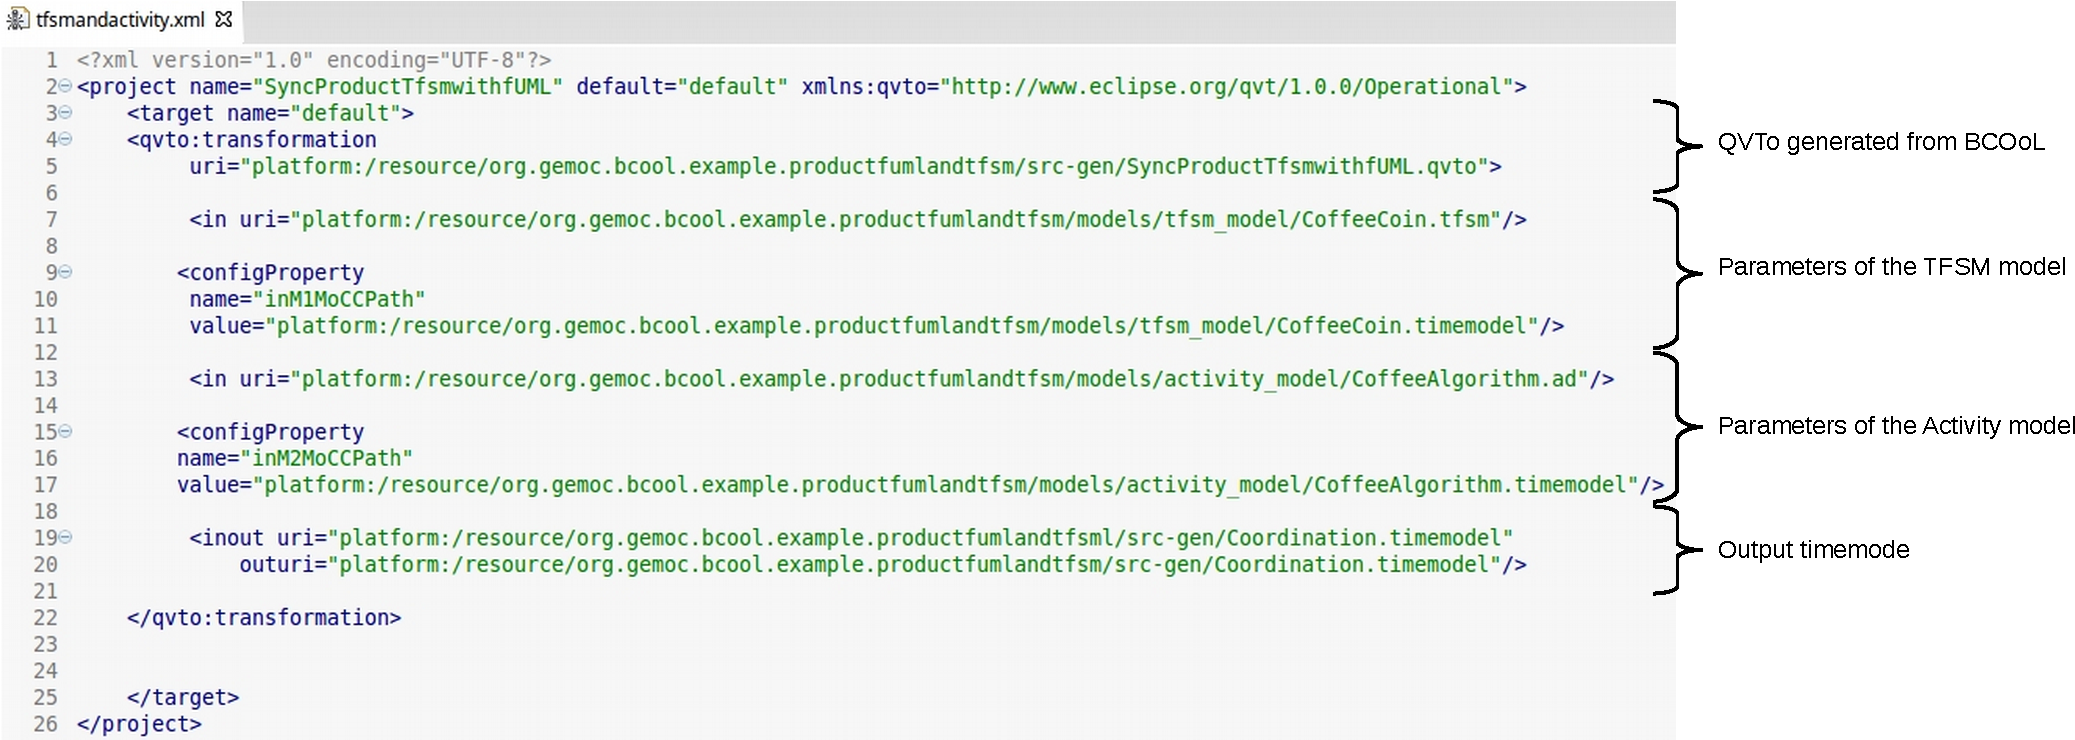
\includegraphics[width=1\textwidth]{bcool/figs/antbcool.pdf}
  %		\caption{ANT script to build the coordination specification for the coffee machine}
  %		\label{fig:screenantbcool}
 % 	\end{center}
 % \end{figure}

